

\documentclass[12pt, a4paper]{report}
\usepackage{epsfig}
\usepackage{subfigure}
%\usepackage{amscd}
\usepackage{amssymb}
\usepackage{graphicx}
%\usepackage{amscd}
\usepackage{amssymb}
\usepackage{subfiles}
\usepackage{framed}
\usepackage{subfiles}
\usepackage{amsthm, amsmath}
\usepackage{amsbsy}
\usepackage{framed}
\usepackage[usenames]{color}
\usepackage{listings}
\lstset{% general command to set parameter(s)
	basicstyle=\small, % print whole listing small
	keywordstyle=\color{red}\itshape,
	% underlined bold black keywords
	commentstyle=\color{blue}, % white comments
	stringstyle=\ttfamily, % typewriter type for strings
	showstringspaces=false,
	numbers=left, numberstyle=\tiny, stepnumber=1, numbersep=5pt, %
	frame=shadowbox,
	rulesepcolor=\color{black},
	,columns=fullflexible
} %
%\usepackage[dvips]{graphicx}
\usepackage{natbib}
\bibliographystyle{chicago}
\usepackage{vmargin}
% left top textwidth textheight headheight
% headsep footheight footskip
\setmargins{3.0cm}{2.5cm}{15.5 cm}{22cm}{0.5cm}{0cm}{1cm}{1cm}
\renewcommand{\baselinestretch}{1.5}
\pagenumbering{arabic}
\theoremstyle{plain}
\newtheorem{theorem}{Theorem}[section]
\newtheorem{corollary}[theorem]{Corollary}
\newtheorem{ill}[theorem]{Example}
\newtheorem{lemma}[theorem]{Lemma}
\newtheorem{proposition}[theorem]{Proposition}
\newtheorem{conjecture}[theorem]{Conjecture}
\newtheorem{axiom}{Axiom}
\theoremstyle{definition}
\newtheorem{definition}{Definition}[section]
\newtheorem{notation}{Notation}
\theoremstyle{remark}
\newtheorem{remark}{Remark}[section]
\newtheorem{example}{Example}[section]
\renewcommand{\thenotation}{}
\renewcommand{\thetable}{\thesection.\arabic{table}}
\renewcommand{\thefigure}{\thesection.\arabic{figure}}
\title{Research notes: linear mixed effects models}
\author{ } \date{ }


\begin{document}
	\author{Kevin O'Brien}
	\title{Mixed Models for Method Comparison Studies}
	\tableofcontents
	
	%----------------------------------------------------------------------------------------%
	\newpage
	\chapter{Techniques for Method Comparison}
	\section{The Bland-Altman Approach to Method Comparison}
	
	%		\citet{BA83} highlighted the inadequacies of these approaches for comparing two methods of measurement, and proposed methods with this specific application in mind. Although the authors also acknowledge the opportunity to apply other, more complex, approaches, but argue that simpler approaches is preferable, especially when the
	%		results must be `explained to non-statisticians'.
The issue of whether two measurement methods comparable to the 	extent that they can be used interchangeably with sufficient accuracy is encountered frequently in scientific research. \citet{BA83} recognized the inadequacies of several analyses and articulated quite thoroughly the basis on which they are unsuitable for comparing two methods of measurement, instead recommending the use of graphical techniques to assess agreement. 



	
In 1983 Bland and Altman published a paper in the Lancet proposing the difference plot for use for method comparison purposes \citep{BA83}. 	Bland-Altman plots are a powerful graphical technique for making
a visual assessment of the data. \citet*{BA83} express the
motivation for this plot:
\begin{quote}
\textit{
	``From this type of plot it is much easier to assess the magnitude
	of disagreement (both error and bias), spot outliers, and see
	whether there is any trend, for example an increase in
	(difference) for high values. This way of plotting the data is a
	very powerful way of displaying the results of a method comparison
	study."}
\end{quote}
 Principally their method is calculating, for each pair of corresponding two methods of measurement of some underlying quantity, with no replicate measurements, the difference $d_i$ and mean $a_i$: case-wise differences of measurements of two methods $d_{i} = x_{i}-y_{i}, \mbox{ for }i=1,2,\dots,n$, on the same subject should be calculated, and then the average of those measurements, $a_{i} = (x_{i} + y_{i})/2 \mbox{ for }i=1,2,\dots, n$. An important requirement is that the two measurement methods use the same scale of measurement. Following a technique known as the Tukey mean-difference plot, as noted by \citet{kozak2014including}, \citet{BA83} proposed that $a_i$ should be plotted against $d_i$, a plot now widely known as the Bland-Altman plot.

%For the Grubbs Data Sets, the relevant calculations are tabulated on Table~\ref{GrubbsData1}, with the resulting plot shown on the right side on Figure~\ref{GrubbsBAcombined}.
%
%	
The case wise-averages capture several aspects of the data, such as expressing the range over which the values were taken, and assessing whether the assumptions of constant variance holds. Case-wise averages also allow the case-wise differences to be presented on a two-dimensional plot, with better data visualization qualities than a one dimensional plot. \citet{BA86}
	cautions that it would be the difference against either measurement value instead of their average, as the difference relates to both value. This approach has proved very popular, and the Bland-Altman plots is widely regarded as powerful graphical tool for making a visual assessment of the data.
	
As the objective of the Bland-Altman plot is to advise on the agreement of two methods, the individual case-wise differences are also particularly relevant. The magnitude of the inter-method bias between the two methods is simply the average of the differences $\bar{d}$, and is represented with a line on the Bland-Altman plot. Further to this method, the presence of constant bias may be indicated if the average value differences is not equal to zero. \citet{BA86} do, however, state that the absence of bias does not provide sufficient information to allow a judgement as to whether or not one method can be substituted for	another.
	
Furthermore they propose their simple approach specifically constructed for method comparison studies. They acknowledge that there are other valid, but complex approaches, but argue that
		a simple approach is preferable,
		\textit{``especially when the results must be explained to
			non-statisticians"} \citep*{BA83}.
		
	\subsection{Inspecting Method Comparison Data}
% - However it is worth mentioning, as it is a simple, powerful and elegant technique that is often overlooked in method comparison studies.
The first step recommended, which the authors argue should be mandatory, is construction of an identity plot, which is a simple scatter-plot approach of measurements for both methods on either axis. The line of equality (the $X=Y$ line, i.e. the 45 degree line through the origin) should also be shown, as it is necessary to give the correct interpretation of how both methods compare. 

This plot can gives the analyst a cursory examination of how well the measurement methods agree. In the case of good agreement, the observations would be distributed closely along the line of equality.  A scatter plot of the Grubbs data is shown on the left in Figure~\ref{GrubbsBAcombined}. Visual inspection confirms the previous conclusion that inter-method bias is present, i.e. the Fotobalk device has a tendency to record a lower velocity.
	
	\begin{figure}[h!]
		\begin{center}
			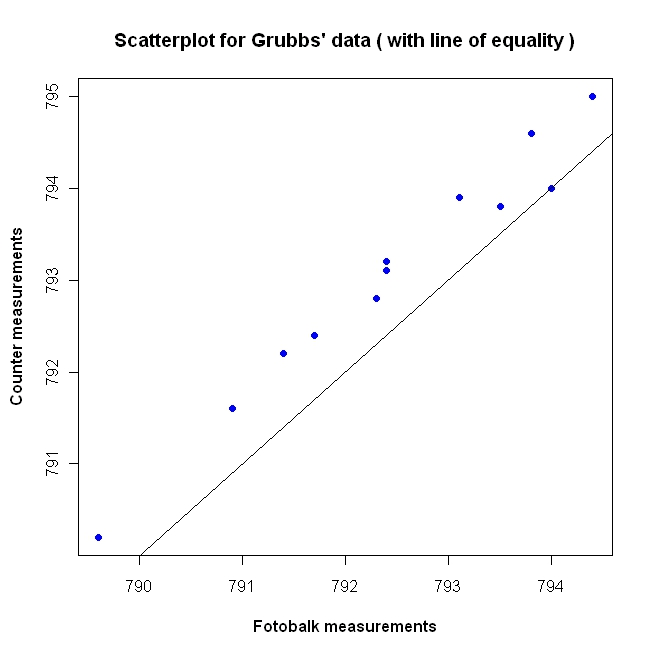
\includegraphics[width=70mm]{images/GrubbsScatter.jpeg}				\includegraphics[width=70mm]{images/GrubbsBAplot-noLOA.jpeg}\\
				\caption{Identity Plot and Bland-Altman Plot For Fotobalk and Counter methods.}\label{GrubbsBAcombined}
			\end{center}
		\end{figure}
	% %	\section{Variations and Alternative Graphical Methods}
	%In this section, we will look at some variations and enhancements of the Bland-Altman plot, as well as some alternative graphcial techniques. 
	% %	Strictly speaking, 
	%%The Identity Plot is advised by Bland and Altman as a prior analysis to the Bland-Alman plot, and therefore is neither a variant nor an alternative approach. 
However scatter-plots, such as these, are not sufficient for a thorough examination of the data. \citet{BritHypSoc} notes that data points will tend to cluster around the line of equality, obscuring interpretation.
	
The Bland-Altman plot for comparing the `Fotobalk' and `Counter' methods, which shall henceforth be referred to as the `F vs C' comparison, is depicted on the right in Figure~\ref{GrubbsBAcombined}, using data from Table~\ref{GrubbsData1}. The dashed line in the Bland-Altman plot alludes to the inter-method bias between the two methods, estimated by calculating the average of the differences. In the case of Grubbs data the inter-method bias is $-0.6083$ metres per second. By inspection of the plot, one would notice that the differences tend to increase as the averages increase.
		
	\begin{table}[h!]
		\renewcommand\arraystretch{0.7}%
		\begin{center}
			\begin{tabular}{|c||c|c|c||c|c|c|c|}
				\hline
				Round & Fotobalk  & Counter & Terma  &   &    &   &   \\
				&  [F] & [C] & [T] &[F-C] &  [(F+C)/2] & [F-T] &  [(F+T)/2] \\
				\hline
				1 & 793.8 & 794.6 & 793.2 & -0.8 & 794.2 & 0.6 & 793.5 \\
				2 & 793.1 & 793.9 & 793.3 & -0.8 & 793.5 & -0.2 & 793.2 \\
				3 & 792.4 & 793.2 & 792.6 & -0.8 & 792.8 & -0.2 & 792.5 \\
				4 & 794.0 & 794.0 & 793.8 & 0.0 & 794.0 & 0.2 & 793.9 \\
				5 & 791.4 & 792.2 & 791.6 & -0.8 & 791.8 & -0.2 & 791.5 \\
				6 & 792.4 & 793.1 & 791.6 & -0.7 & 792.8 & 0.8 & 792.0 \\
				7 & 791.7 & 792.4 & 791.6 & -0.7 & 792.0 & 0.1 & 791.6 \\
				8 & 792.3 & 792.8 & 792.4 & -0.5 & 792.5 & -0.1 & 792.3 \\
				9 & 789.6 & 790.2 & 788.5 & -0.6 & 789.9 & 1.1 & 789.0 \\
				10 & 794.4 & 795.0 & 794.7 & -0.6 & 794.7 & -0.3 & 794.5 \\
				11 & 790.9 & 791.6 & 791.3 & -0.7 & 791.2 & -0.4 & 791.1 \\
				12 & 793.5 & 793.8 & 793.5 & -0.3 & 793.6 & 0.0 & 793.5 \\
				\hline
			\end{tabular}
			\caption{Fotobalk : Differences and Averages with Counter and Terma.}
			\label{GrubbsData1}
		\end{center}
	\end{table}

In Figure~\ref{GrubbsDataTwoBAplots} Bland-Altman plots for the `F vs C' and `F vs T'
	comparisons are shown, where `F vs T' refers to the comparison of
	the `Fotobalk' and `Terma' methods. Usage of the Bland-Altman plot
	can be demonstrate in the contrast between these comparisons. By inspection, there exists a larger inter-method bias in the `F vs C' comparison than in the `F vs T' comparison. Conversely there appears to be less precision in `F vs T' comparison, as indicated by the greater dispersion of covariates.
	
	\begin{figure}[h!]
		\begin{center}
			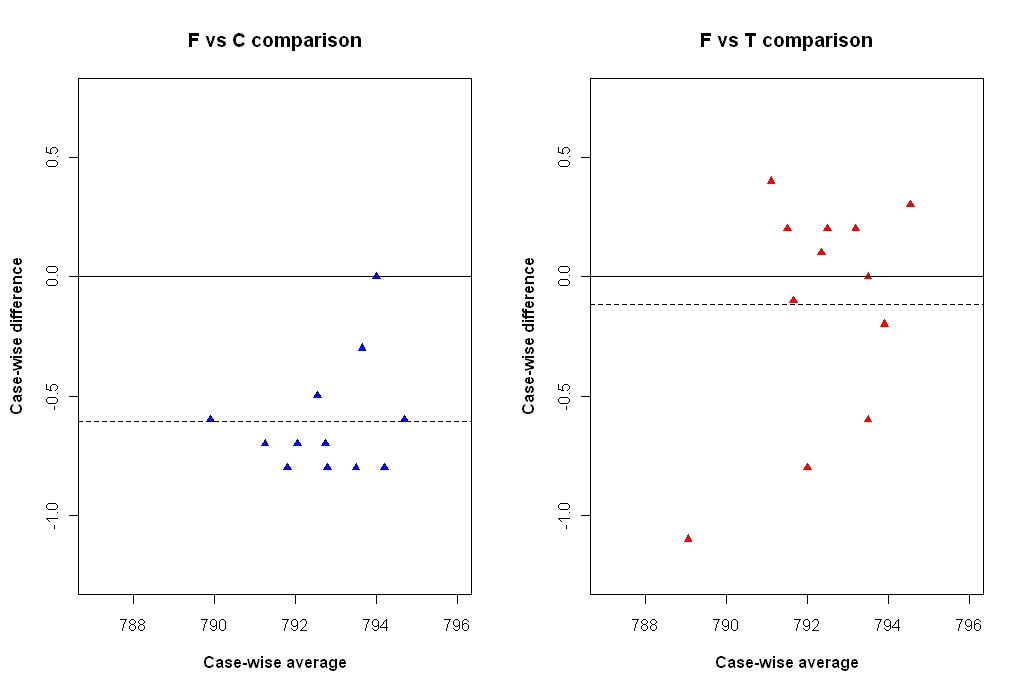
\includegraphics[height=100mm]{images/GrubbsDataTwoBAplots.jpeg}
			\caption{Bland-Altman plots for Grubbs' F vs C and F vs T comparisons.}\label{GrubbsDataTwoBAplots}
		\end{center}
	\end{figure}
	

	
	
	%\subfile{TechAcceptModel.tex}
	
	
	%\begin{figure}[h!]
	%	\begin{center}
	%		\includegraphics[width=120mm]{GrubbsBAplot-noLOA.jpeg}
	%		\caption{Bland-Altman plot For Fotobalk and Counter methods.}\label{GrubbsBA-noLOA}
	%	\end{center}
	%\end{figure}
	
	
	
	%	\section{scatter plots} The authors advise the
	%	use of scatter plots to identify outliers, and to determine if
	%	there is curvilinearity present. In the region of linearity
	%	,simple linear regression may yield results of interest.
	




Estimates for inter-method bias and variance of differences are only meaningful if there is uniform inter-bias and variability throughout the range of measurements. Fulfilment of these assumptions can be checked by visual inspection of the Bland-Altman plot.

% % The prototype Bland-Altman plots depicted in Figures 1.4, 1.5 and 1.6 are derived from simulated data, for the purpose of demonstrating how the plot would inform an analyst of features that would adversely affect use of the recommended approach.
	
Figure~\ref{BAFanEffect} and Figure~\ref{PropBias} show two Bland-Altman plots derived from
	simulated data, each for the purpose of demonstrating how the plot would inform an analyst of trends that would adversely affect use of the recommended approach. Additionally the procedure is not properly constructed to deal with outliers, which  shall be reverted to later.
	
Figure~\ref{BAFanEffect} demonstrates how the Bland-Altman plot would indicate
	increasing variance of differences over the measurement range.
	Fitted regression lines, for both the upper and lower half of the	plot, have  been added to indicate the trend. Application of regression techniques to the Bland-Altman plot, and subsequent formal testing for the constant variability of differences is informative. The data set may be divided into two subsets, containing the observations wherein the difference values are less than and greater than the inter-method bias respectively. For both of these fits, hypothesis tests for the respective slopes can be performed. While both tests could be considered separately, multiple comparison procedures are advisable, for example, the Benjamini-Hochberg Test \citep{BH}.
	
Figure~\ref{PropBias} is an example
	of cases where the inter-method bias changes over the measurement range. This is known as proportional bias, and is defined by \citet{ludbrook97} as meaning that `\textit{one method gives
	values that are higher (or lower) than those from the other by an
	amount that is proportional to the level of the measured variable}'. Both of these cases violate the assumptions necessary for further analysis using limits of agreement, which shall be discussed later. 
	
	\begin{figure}[h!]
		\begin{center}
			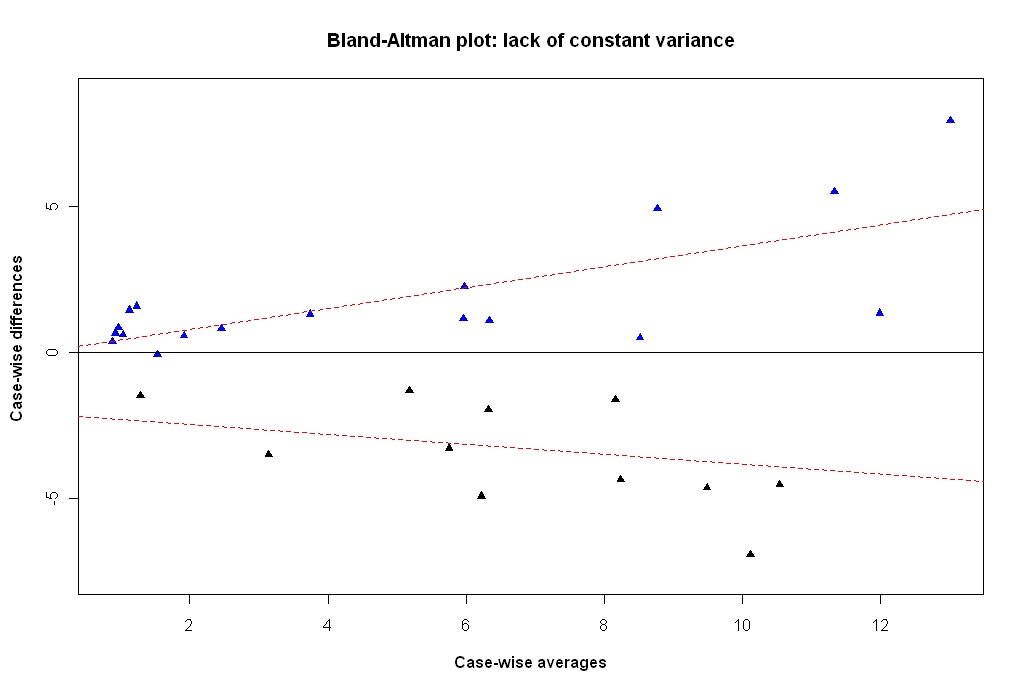
\includegraphics[width=110mm]{images/BAFanEffect.jpeg}
			\caption{Bland-Altman Plot demonstrating the increase of variance over the range}\label{BAFanEffect}
		\end{center}
	\end{figure}
	
\begin{figure}[h!]
\begin{center}
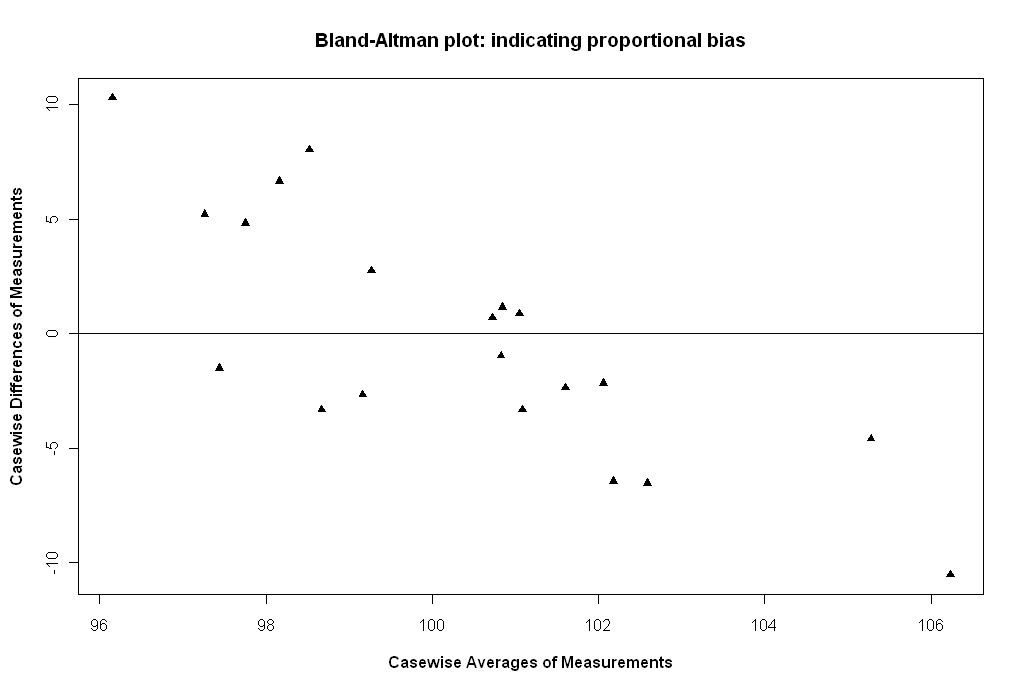
\includegraphics[width=110mm]{images/PropBias.jpeg}
\caption{Bland-Altman Plot indicating the presence of proportional bias}\label{PropBias}
\end{center}
\end{figure}
Due to limitations of the conventional difference plot, a series of alternative formulations for the Bland-Altman approach have been proposed. Referring to the assumption that bias and variability are constant across the range of measurements, \citet{BA99} address the case where there is an increase in variability as the magnitude increases. They remark that it is possible to ignore the issue altogether, but the limits of agreement would be wider apart than necessary when just lower magnitude measurements are considered. Conversely the limits would be too narrow should only higher magnitude measurements be used. 
	
	To address the issue, they propose the logarithmic transformation of the data. The plot is then formulated as the difference of paired log values against their mean. Bland and Altman acknowledge that this is not easy to interpret, and may not be suitable in all cases.
	
	\citet{BA99} offers two variations of the Bland-Altman plot that are intended to overcome potential problems that the conventional plot would be inappropriate for. The first variation is a plot of case-wise differences as percentage of averages, and is appropriate when there is an increase in variability of the differences as the magnitude increases. 
	
	The second variation is a plot of case-wise ratios as percentage of averages, removing the need for logarithmic transformation. This approach is useful when there is an increase in variability of the differences as the magnitude of the measurement increases. \citet{Eksborg} proposed such a ratio plot, independently of Bland and Altman. \citet{Dewitte} commented on the reception of this article by saying `\textit{Strange to say, this report has been overlooked}'.
	
\section{Limits of Agreement}
% introduces
A third element of the Bland-Altman approach, an interval known
as limits of agreement is introduced in \citet*{BA86} (sometimes referred to in literature as 95\% limits of agreement). These limits centre on the
average difference line, and are computed as $LOA = \bar{d} \pm 1.96 s_{d}$
with $\bar{d}$ as the estimate of the inter method bias and $s_{d}$ the standard deviation of the differences. Limits of agreement are used to assess whether the two methods of measurement can be used interchangeably, by demonstrating the range in which 95\% of the sample data should lie.  The limits of agreement requires an assumption of a constant level of bias throughout the range of measurements. 





\citet{BA86} refer to
this as the `equivalence' of two measurement methods. The specific purpose of the limits of
agreement must be
established clearly. \citet*{BA95} comment that the limits of agreement
\textit{`how
	far apart measurements by the two methods were likely to be for
	most individuals}', a definition echoed in their 1999 paper:

\begin{quote}
\textit{We can then say that nearly all pairs
	of measurements by the two methods will be closer together than
	these extreme values, which we call 95\% limits of agreement.
	These values define the range within which most differences
	between measurements by the two methods will lie.}
\end{quote}

Importantly the authors recommend prior determination of what would constitute acceptable agreement, and that sample sizes should be predetermined to give an accurate conclusion. However, \citet{mantha} highlight inadequacies in the correct application of limits of agreement, resulting in contradictory estimates of limits of agreement in various papers.


Calculation of the limits of agreement relies on the assumption that the case-wise differences are normally distributed, although the measurements themselves are not assumed to follow any distribution. This assumption is justified because variation between subjects has been removed, leaving measurement error, which is likely to be normally distributed \citep{BA86}. \citet{BA99} remark that this assumption is easy to check using commonly used methods, i.e. a normal probability plot. 

For the Grubbs `F vs C' comparison, these limits of agreement are calculated as -0.132 for the upper bound, and -1.08 for the lower bound. Figure~\ref{GrubbsBAplot-noLOA} shows the resultant Bland-Altman plot, with the limits of agreement shown in dotted lines.

\begin{figure}[h!]
	\begin{center}
		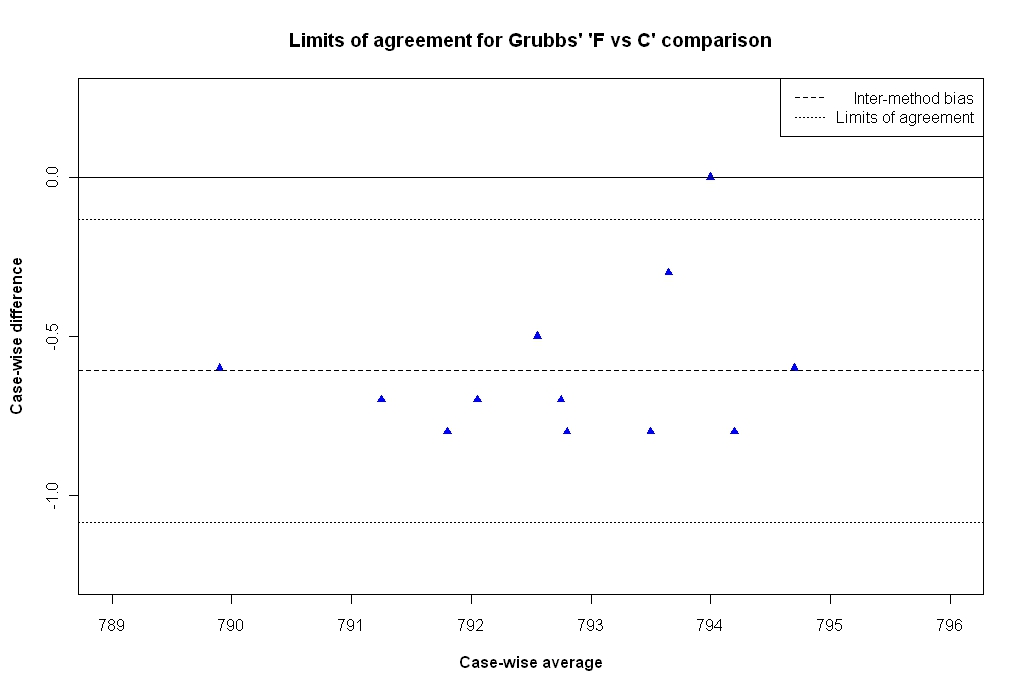
\includegraphics[width=125mm]{images/GrubbsBAplot-LOA.jpeg}
		\caption{Bland-Altman plot with limits of agreement}
		\label{GrubbsBAplot-noLOA}
	\end{center}
\end{figure}

\subsection{Interpretation of Limits Of Agreement}

%
%As \citet*{BA86} point
%out this may not be the case. Bland and Altman advises on how to
%calculate of confidence intervals for the inter-method bias and
%the limits of agreement. 

%\subsubsection{Small Sample Sizes} The limits of agreement are
%estimates derived from the sample studied, and will differ from
%values relevant to the whole population, hence the importance of a
%suitably large sample size. A different sample would give
%different limits of agreement. Student's t-distribution is a well
%known probability distribution used in statistical inference for
%normally distributed populations when the sample size is small
%\citep{student,Fisher3}. Consequently, using 't' quantiles , as
%opposed to standard normal quantiles, may give a more appropriate
%calculation for limits of agreement when the sample size is small.
%For sample size $n=12$ the `t' quantile is 2.2 and the limits of
%agreement are (-0.074,-1.143).

\citet{BA99} note the similarity of limits of agreement to
confidence intervals, but are clear that they are not the same thing. Interestingly, they describe the limits as `\textit{being like a reference interval}', offering no elaboration.

The Shewhart chart is a well known graphical
technique used in statistical process control. Consequently
there is potential for misinterpreting the limits of agreement as
if they were Shewhart control limits. Importantly the
parameters used to determine the limits, the mean and standard
deviation, are not based on any randomly ordered sample used for an analysis, but on a statistical process's time ordered values, a key difference with Bland-Altman limits of agreement.

%\citet{BXC2008} offers an alternative, more specific,  definition of
%the limits of agreement \emph{"a prediction interval for the
%	difference between future measurements with the two methods on a
%	new individual."}

\citet{BXC2008} regards the limits of agreement as a prediction interval for the difference between future measurements with the two methods on a new individual, but states that it does not fit the formal definition of a prediction interval, since the
definition does not consider the errors in estimation of the parameters. 

Prediction intervals, which are often used in regression analysis, are estimates of an interval in which future
observations will fall, with a certain probability, given what has already been observed. \citet{BXC2008} offer an alternative
formulation, a $95\%$ prediction interval for the difference
\begin{equation}
\bar{d} \pm t_{(0.025, n-1)}S_{d} \sqrt{1+\frac{1}{n}}
\end{equation}

%\noindent where $n$ is the number of subjects. Only for 61 or more
%subjects is there a quantile less than 2.
 where $n$ is the number of subjects. With consideration of the effect of the sample size on the interval
width, \citet{BXC2008} remarks that only for 61 or more subjects is the quantile less than 2.

\citet{luiz} describes limits of agreement as tolerance limits. A
tolerance interval for a measured quantity is the interval in
which a specified fraction of the population's values lie, with a
specified level of confidence. \citet{luiz} offers an alternative description of limits of agreement, this time as tolerance limits. 

\citet{Barnhart} describes them as a probability interval, and offers a clear description of how they should be used; `\textit{if the absolute limit is less than an acceptable difference $d_{0}$, then the agreement between the two methods is deemed satisfactory}'.

Various other interpretations as to how limits of agreement should properly be defined. The prevalence of contradictory definitions of what limits of agreement strictly will inevitably attenuate the poor standard of reporting using limits of agreement, as discussed by \citet{mantha}.

%At least 100 historical
%values must be used to determine the acceptable value (i.e the
%process mean) and the process standard deviation. The principle
%that the mean and variance of a large sample of a homogeneous
%population is a close approximation of the population's mean and
%variance justifies this.



\subsection{Precision of Limits of Agreement}

The limits of agreement are estimates derived from the sample studied, and will differ from values relevant to the whole
population. \citet*{BA86} advance a formulation for confidence
intervals of the inter-method bias and the limits of agreement, arguing that it is possible to make such estimates if it is assumed that the case-wise differences approximately follow a normal distribution. However \citet*{BA99} caution that such calculations may be `somewhat
optimistic' if the associated assumptions are not valid. A $95\%$ confidence interval can be determined, by means of the
\emph{t} distribution with $n-1$ degrees of freedom. For the inter-method bias, the confidence interval is simply that of a mean: $\bar{d} \pm t_{(\alpha/2,n-1)} S_{d}/\sqrt{n}$.

The confidence intervals and standard error for the limits of agreement follow from the variance of the limits of agreement, which is shown to be

\[
\operatorname{Var}(LOA) = \bigg(\frac{1}{n}+\frac{1.96^{2}}{2(n-1)}\bigg)s_{d}^{2}.
\]

If $n$ is sufficiently large this can be following approximation can be used
\[
\mbox{Var}(LOA) \approx 1.71^{2}\frac{s_{d}^{2}}{n},
\]
with the standard errors of both limits can be approximated as $1.71$ times the standard error of the differences.

%%%%%%%%%%%%%%%%%%%%%%%%%%%%%%%%%%%%%%%%%%%%%%%%%%%%%%%%%%%%%%%%%%%%%%%%%%%%%%%%%%%%%%


\section{Detection of Outliers in the Bland-Altman Framework}
%As with the Bland-Altman plot, the formulation of the Limits of Agreement is also heavily influenced by outliers. An example
%in \citet*{BA83} demonstrates the effect of recalculating without
%a particular outlier. Refering to the VCF data set in the same
%paper, there is more than one outlier.

The Bland-Altman plot can be used to identify outliers. Here  we use a simple definition of an outlier as an observation that is conspicuously different from the rest of the data that it arouses suspicion that it occurs due to a mechanism, or conditions, different to that of the rest of the observations. In their 1983 paper they merely state that the plot can be used to
``spot outliers". In their 1986 paper, Bland and Altman give an example of an
outlier. They state that it could be omitted in practice, but make
no further comments on the matter. In \citet{BA99}, we get the clearest indication of
what they suggest on how to react to the presence of
outliers. Their recommendation is to recalculate the limits
without them, in order to test the difference with the calculation
where outliers are retained. \citet*{BA99} do not recommend excluding outliers from analyses. However recalculation of the inter-method bias estimate, and further calculations based upon that estimate, are useful for assessing the influence of outliers. \citet{BA99} states that \emph{``We usually find that this method of analysis is not too sensitive to one or two large outlying differences."}
Classification thereof is a subjective decision in any analysis, but must be informed by the logic of the mechanism that produces the data.. Figure~\ref{BAOutliers} is a Bland-Altman plot with two conspicuous observations, at the extreme left and right of the
plot respectively. 
\begin{figure}[h!]
		\begin{center}
			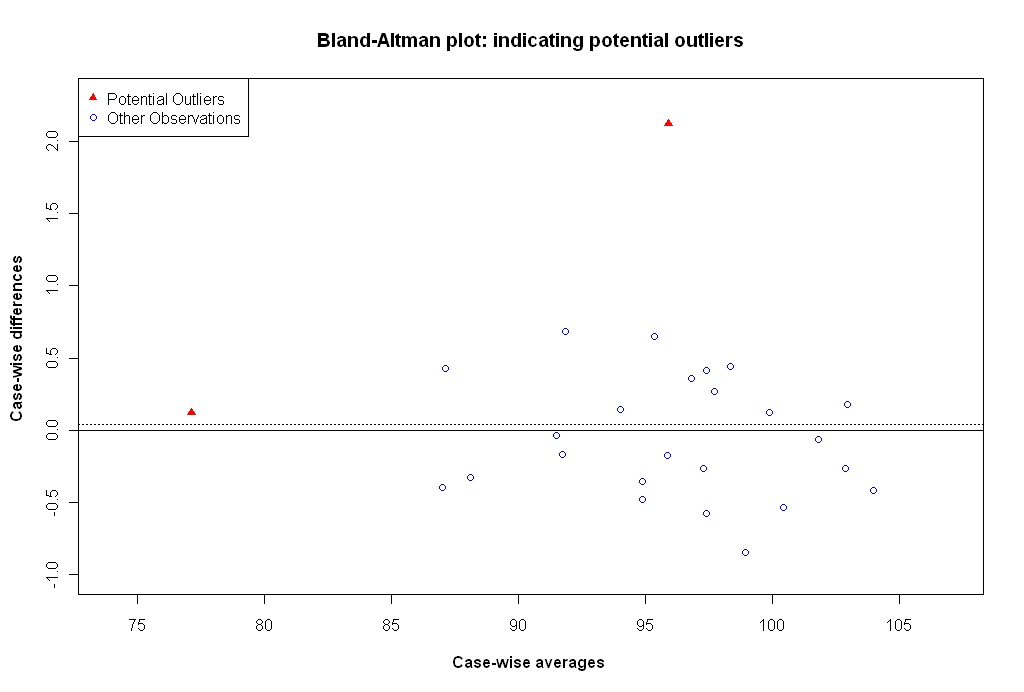
\includegraphics[width=125mm]{images/BAOutliers.jpeg}
			\caption{Bland-Altman plot indicating the presence of outliers}\label{BAOutliers}
		\end{center}
	\end{figure}
In the Bland-Altman plot depicted in Figure~\ref{BAOutliers}, consider the covariate located on the extreme left of the plot. Ordinarily we would conclude that this point due to it's horizontal displacement from the main cluster of points. However this horizontal displacement is supported by two independent measurements and is very close to the inter-method bias, i.e. very close to its expected value. Therefore that observation, should not be considered an outlier at all.

Conversely the observation located at the top of the plot, should be considered an outlier, as it has a noticeable vertical displacement from the rest of the observations. There are no mitigating factors.

\subsection{Bartko's Ellipse}

As an enhancement on the Bland-Altman Plot, \citet{Bartko} has
expounded a confidence ellipse for the covariates. \citet{Bartko} offers a graphical complement to the Bland-Altman
plot in the form of a bivariate confidence ellipse as a boundary for dispersion, with \citet{AltmanEllipse} providing the relevant calculations. This ellipse is intended as a visual guideline for the scatter plot, for detecting outliers and to assess the within- and between-subject variability. The stated purpose is to `amplify dispersion', which presumably is for the purposes of outlier detection. The orientation of the the ellipse is key to interpreting the results. Additionally Bartko's ellipse provides a visual aid to determining the relationship between variances. 
\begin{center}
\begin{figure}[h!]
	% Requires \usepackage{graphicx}
	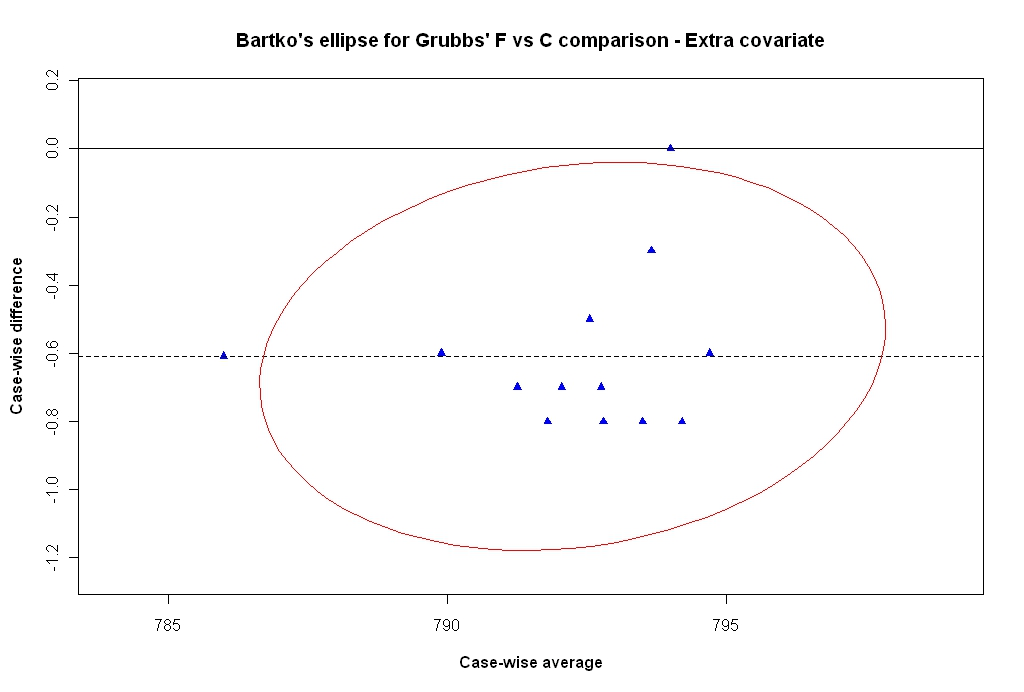
\includegraphics[width=130mm]{images/GrubbsBartko2.jpeg}
	\caption{Bartko's ellipse for Grubbs data}\label{GrubbsBartko2}
\end{figure}
\end{center}
The minor axis relates to the between-subject variability, whereas the major axis relates to the error mean square, with the ellipse depicting the size of both relative to each other.

Furthermore, the ellipse provides a visual aid to determining the relationship between the variance of the means $\operatorname{Var}(a)$ and the variance of the differences $\operatorname{Var}(d)$. If $\operatorname{Var}(a)$ is greater than $\operatorname{Var}(d)$, the orientation of the ellipse is horizontal. Conversely if $\operatorname{Var}(a)$ is less than $\operatorname{Var}(d)$, the orientation of the ellipse is vertical. The more horizontal the ellipse, the greater the degree of agreement between the two methods being tested.


%(Furthermore \citet{Bartko}
%proposes formal testing procedures, that shall be discussed in due
%course.)
Bartko states that the ellipse can, inter alia, be used to detect the presence of outliers. The limitations of using bivariate approaches to outlier detection in the Bland-Altman plot can demonstrated using Bartko's ellipse.


The Bland-Altman plot for the Grubbs data, complemented by Bartko's ellipse, is depicted in Figure~\ref{GrubbsBartko2}. However, both observation that were previously considered as potential outliers (i.e. the extreme left and the uppermost) are shown to be outside the bounds of the ellipse, indicating both to be outliers.

%----------------------------------------------------------------------------%
\subsection{Grubbs' Test for Outliers}

In classifying whether an observation from a univariate data set is an outlier, many formal tests are available, such as the Grubbs test for outliers. In assessing whether a covariate in a Bland-Altman plot is an outlier, this test is useful when applied to the case-wise difference values treated as a univariate data set. The null hypothesis of the Grubbs test procedure is the absence of any outliers in the data set. 

The test statistic for the Grubbs test ($G$) is the largest absolute deviation from the sample mean divided by the standard
deviation of the differences,
\begin{equation}
G =  \displaystyle\max_{i=1,\ldots, n}\frac{\left \vert d_i -
	\bar{d}\right\vert}{S_{d}}.
\end{equation}

For the `F vs C' comparison it is the fourth observation that gives rise to the test statistic, $G = 3.64$. The critical value is
calculated using Student's $t$ distribution and the sample size,
\[
U = \frac{n-1}{\sqrt{n}} \sqrt{\frac{t_{\alpha/(2n),n-2}^2}{n - 2
		+ t_{\alpha/(2n),n-2}^2}}.
\]
For this test $U = 0.75$. The conclusion of this test is that the fourth observation in the `F vs C' comparison is an outlier, with $p-$value = 0.003, in accordance with the previous result of Bartko's ellipse.


\section{Prevalence of the Bland-Altman Plot}

\citet*{BA86}, which further develops the Bland-Altman approach,
was found to be the sixth most cited paper of all time by \citet{BAcite}. \cite{Dewitte} reviews the use of Bland-Altman plots by examining all articles in the journal `Clinical Chemistry' between 1995 and 2001, describing the rate at which
prevalence of the Bland-Altman plot has developed in scientific
literature. This study concludes that use of the Bland-Altman plot increased over the years, from 8\% in 1995 to
14\% in 1996, and 31-36\% in 2002.

The Bland-Altman plot has since become the expected, and often the obligatory, approach for presenting method comparison
studies in many scientific journals \citep{hollis}. Furthermore \citet{BritHypSoc} recommend its use in papers pertaining to
method comparison studies for the journal of the British Hypertension Society.


% %	\section{Bland Altman Plots In Literature}
\citet{mantha} contains a study on the use of Bland Altman plots of 44 articles in several named journals over a two year period. 42 articles used Bland Altman's limits of agreement, while the other two used correlation and regression analyses. \citet{mantha} remark that 3 papers, from 42 mention predefined maximum width for limits of agreement that would not impair medical care.

The conclusion of \citet{mantha} is that there are several inadequacies and inconsistencies in the reporting of results, and
that more standardization in the use of Bland-Altman plots is required. The authors recommend the prior determination of limits of agreement before the study is carried out. This contention is endorsed by \citet{lin}, which makes a similar recommendation for the sample size, noting that\emph{``sample sizes required either was not mentioned or no rationale for its choice was given"}.

\begin{quote}
\textit{In order to avoid the appearance of ``data dredging", both the
	sample size and the (limits of agreement) should be specified and
	justified before the actual conduct of the trial.} \citep{lin}
\end{quote}

\citet{Dewitte} remark that the limits of agreement should be
compared to a clinically acceptable difference in measurements.

\section{Criticism of Limits of Agreement}
The Bland-Altman approach is well noted for its ease of use, and can be easily implemented with most software packages. Also it does not require the practitioner to have more than basic statistical training. The plot is quite informative about the variability of the differences over the range of measurements. For
example, an inspection of the plot will indicate the `fan effect' or the presence of an outlier.





%
%
%How this relates the overall population is unclear. It seems that
%it depends on an expert to decide whether or not the range of
%differences is acceptable. In a study A Bland-Altman plots compare
%two assay methods. It plots the difference between the two
%measurements on the Y axis, and the average of the two
%measurements on the X axis

However the approach comes in for criticism in a number of respects. In the first instance, some caution must be given to the inter-method bias estimate.
If one method is sometimes higher, or sometimes lower, the average of the differences will be close to zero. If the inter-method bias is close to zero, there be an indication that the two measurement methods are in agreement, when in fact they are producing different results systematically.

Several problems have been highlighted regarding limits of agreement. One is the somewhat arbitrary manner in which they are constructed. Limits of agreement are intended to analyse equivalence. How this is assessed is the considered judgement of the practitioner. In \citet{BA86} an example of good agreement is cited. For two methods of measuring `oxygen saturation', the limits of agreement are calculated as (-2.0,2.8) percentage points. According to the authors, a knowledgeable practitioner in the field should ostensibly find this to be sufficiently narrow. If the limits of agreement are not clinically important, which is to say that the differences tend not to be substantial, the two methods may be used interchangeably. Furthermore \citet{DunnSEME} takes issue
with the notion of `equivalence', remarking that while agreement
indicated equivalence, equivalence does not reflect agreement.


While in essence they are similar to confidence intervals, limits of agreement are not constructed as such; they are designed for future values. Lack of clarity in this regards can give rise to confusion, and incorrect interpretations.

\citet{ludbrook97,ludbrook02} criticizes Bland-Altman plots on the basis that they present no information on effect of constant bias or proportional bias. These plots are only practicable when both methods measure in the same units, hence they are totally
unsuitable for conversion problems. There is no guidance on how to deal with outliers. Bland and Altman recognize the effect they would have on the limits of agreement, but offer no guidance on how to correct for those effects. Finally the adaptation of the approach to deal with replicate measurements, as specified by \citet{BA99}, is flawed.

\section{Limits of Agreement for Replicate Measurements}

Computing limits of agreement features prominently in many method comparison studies since the publication of \citet{BA86}.
\citet{BA99} addresses the issue of computing LOAs in the presence of replicate measurements, suggesting several computationally simple approaches. When repeated measures data are available, it is desirable to use
all the data to compare the two methods. However, the original Bland-Altman method was developed for two sets of measurements done on one occasion, and so this approach is not suitable for replicate measures data. However, as a naive analysis, it may be used to explore the data because of the simplicity of the method.
Contrary to \citet{BA99}, \citet{BXC2008} computes the limits of agreement to the case with replicate measurements by using LME models. This approach will be discussed in due course.




\section{Formal Models and Tests}
While the Bland-Altman plot is a simple technique for comparing measurements, \citet{Kinsella} noted the lack of formal testing offered by
that approach, with it relying on the practitioner's opinion to judge the outcome. \citet{BA83} proposed a formal test on the
Pearson correlation coefficient of case-wise differences and means which, according to the authors, is equivalent
to the `Pitman-Morgan Test', a key contribution to method comparison studies that shall discussed shortly \citep{morgan, pitman}. There has been no further mention of this particular test in
\citet{BA86}, although \citet{BA99} refers to Spearman's rank
correlation coefficient. \citet{BA99} remarked that`\textit{we do not see a
	place for methods of analysis based on hypothesis testing}', while also stating that they consider structural equation models to be inappropriate.

%
%For the Grubbs data, the correlation
%coefficient estimate ($r_{(a,d)}$) is 0.2625, with a 95\% confidence
%interval of (-0.366, 0.726) estimated by Fishers `$r$ to $z$'
%transformation \citep*{cohen2013applied}. The null hypothesis ($\rho_{AD}$ =0)
%fail to be rejected. Consequently the null hypothesis of equal
%variances of each method would also fail to be rejected. 
\subsection{Kinsella's Model}
\citet{Kinsella} presented a simple model to describe a measurement by each method, describing the relationship with its real value. Only the non-replicate case is considered, as this is the context of the Bland-Altman plots. Other authors, such as \citet{BXC2004,BXC2008}, present similar formulations of the same model, as well as modified models to account for multiple measurements by each methods on each item, known as replicate measurements.

\citet{Kinsella} formulates a model for
single measurement observations for a method comparison study as a
linear mixed effects model, i.e. model that additively combine
fixed effects and random effects.
\[
Y_{ij} =\quad \mu + \beta_{j} + u_{i} + \epsilon_{ij} \qquad i = 1,\dots,n
\qquad j=1,2\]
The true value of the measurement is represented by $\mu$ while the fixed effect due to method $j$ is $\beta_{j}$.
For simplicity these terms can be combined into single terms; $\mu_{1} = \mu+ \beta_{1}$ and $\mu_{2} = \mu + \beta_{2}$. The inter-method bias is the difference of the two fixed effect terms, $ \mu_d = \beta_{1}-\beta_{2}$. Each of the $i$ items are assumed to give rise to random error, represented by $u_{i}$. This random effects terms is assumed to have mean zero and be normally distributed with variance $\sigma^2$. There is assumed to be an attendant error for each measurement on each item, denoted $\epsilon_{ij}$, which is also assumed to have mean zero. The variance of measurement error for both methods are not assumed to be identical for both methods variance, hence it is denoted $\sigma^2_{j}$. The set of observations ($x_{i},y_{i}$) by methods $X$ and $Y$ are assumed to follow the bivariate normal distribution with expected values $E(x_{i})= \mu_{1}$ and $E(y_{i})= \mu_{2}$ respectively. The variance covariance of the observations $\Sigma$ is given by
\[
\Sigma_{(X,Y)} = \left[
\begin{array}{cc}
\sigma^{2} + \sigma^{2}_{1} & \sigma^{2} \\
\sigma^{2} & \sigma^{2} + \sigma^{2}_{2} \\
\end{array}
\right].
\]

The case-wise differences and means are calculated as $d_{i} =
x_{i}-y_{i}$ and $a_{i} = (x_{i}+y_{i})/2$  respectively.  Both
$d_{i}$ and $a_{i}$ are assumed to follow a bivariate normal
distribution with $E(d_{i})= \mu_{d} = \mu_{1} - \mu_{2}$ and
$E(a_{i})= \mu_{a} = (\mu_{1} + \mu_{2})/2$. Constructively, the paired measurements can be expressed as
\[ d_{i} = x_{i} - y_{i} \sim \mathcal{N} (\mu_d, \sigma^2_{1} + \sigma^2_{2}). \] The variance matrix
$\Sigma_{(A,D)}$ is
\begin{eqnarray}
\Sigma_{(A,D)}= \left[\begin{matrix}
\sigma^{2}_{1}+\sigma^{2}_{2}&\frac{1}{2}(\sigma^{2}_{1}-\sigma^{2}_{2})\\
\frac{1}{2}(\sigma^{2}_{1}-\sigma^{2}_{2})&\sigma^{2}+
\frac{1}{4}(\sigma^{2}_{1}+\sigma^{2}_{2})
\end{matrix} \right].
\end{eqnarray}

%Importantly, this is independent of the true value $\mu$. As the case-wise differences are of interest, the main parameter of interest is the inter-method bias fixed effects for methods $\mu_d = \beta_1-\beta_2$.

%\citet{BXC2010} presents a useful formulation
%	\begin{eqnarray} X_i = \tau_i + \delta_i, \phantom{spacin} \delta_i \sim \mathcal{N}(0,\sigma^2_\delta)\\ Y_i = \alpha + \beta \tau_i + \epsilon_i, \phantom{spaci}  \epsilon_i \sim \mathcal{N}(0,\sigma^2_\epsilon)\end{eqnarray}
%	

In some types of analysis, such as the conversion problems described by \citet{lewis}, measurements made by methods $X$ and $Y$ may be denominated in different units, and an estimate for the proportionality, i.e. a scaling factor, must be determined. Using amended notation, for comparing two methods $X$ and $Y$, for the measurement of item $i$ is formulated as
\begin{eqnarray}
X_i = \tau_i + \epsilon_{i1}, \phantom{spacin} \epsilon_{i1} \sim \mathcal{N}(0,\sigma^2_1),\\
Y_i = \alpha + \lambda \tau_i + \epsilon_{i2}, \phantom{spaci}  \epsilon_{i2} \sim \mathcal{N}(0,\sigma^2_2).
\end{eqnarray}
Here the unknown `true value' is $\tau_i$, $\alpha$ represents the inter-method bias, and the scaling factor is denoted here as $\lambda$. For the time being, we will restrict ourselves to problems where $\lambda$ is assumed to be 1, but will revert back to this conversion problem later. 


\citet{Kinsella} demonstrates the estimation of the variance terms and relative precisions relevant to a method comparison study, with attendant confidence intervals for both. The measurement model introduced by \citet{Grubbs48,Grubbs73} provides a formal procedure for estimate the variances $\sigma^2$, $\sigma^2_{1}$ and $\sigma^2_{2}$ devices. \citet{Grubbs48} offers maximum likelihood estimates, commonly known as Grubbs estimators, for the various variance components, 
\begin{eqnarray*}
	\hat{\sigma^{2}} = \sum{\frac{(x_{i}-\bar{x})(y_{i}-\bar{y})}{n-1}} = Sxy,\\
	\hat{\sigma^{2}_{1}} = \sum{\frac{(x_{i}-\bar{x})^{2}}{n-1}} =S^{2}x - Sxy,  \\
	\hat{\sigma^{2}_{2}} =
	\sum{\frac{(y_{i}-\bar{y})^{2}}{n-1}} = S^{2}y - Sxy.
\end{eqnarray*}

% The standard error of these variance estimates are:
% \begin{eqnarray}
% \mbox{var}(\sigma^{2}_{1}) = \frac{2\sigma^{4}_{1}}{n-1} +
% \frac{\sigma^2_{S}\sigma^2_{1}+\sigma^2_{S}\sigma^2_{2}+\sigma^2_{1}\sigma^2_{2}
% }{n-1}\\
% \mbox{var}(\sigma^{2}_{2}) =\quad \frac{2\sigma^{4}_{2}}{n-1} +
% \frac{\sigma^2_{S}\sigma^2_{1}+\sigma^2_{S}\sigma^2_{2}+\sigma^2_{1}\sigma^2_{2}
% }{n-1}\nonumber
% \end{eqnarray}

\citet{Thompson} presents confidence intervals for the relative
precisions of the measurement methods, $\Delta_{j}=
\sigma^2_{S}/\sigma^2_{j}$ (where $j=1,2$), as well as the
variances $\sigma^{2}_{S}, \sigma^{2}_{1}$ and $\sigma^{2}_{2}$,
\begin{eqnarray}
\Delta_{1} >\quad \frac{C_{xy}-
	t(|A|/n-2))^{\frac{1}{2}}}{C_{x}-C_{xy}+
	t(|A|/n-2))^{\frac{1}{2}}}.
\end{eqnarray}
\citet{Thompson} defines $\Delta_{j}$ to be a measure of the
relative precision of the measurement methods, with $\Delta_{j}=
\sigma^2/\sigma^2_{j}$. Thompson also demonstrates how to make statistical inferences about $\Delta_{j}$.
Based on the following identities,
\begin{eqnarray*}
	C_{x}&=&(n-1)S^2_{x},\nonumber\\
	C_{xy}&=&(n-1)S_{xy},\nonumber\\
	C_{y}&=&(n-1)S^2_{y},\nonumber\\
	|A| &=& C_{x}\times C_{y} - (C_{xy})^2,\nonumber
\end{eqnarray*}
\noindent the confidence interval limits of $\Delta_{1}$ are
\begin{eqnarray}
\Delta_{1} < \frac{C_{xy}-
	t(\frac{|A|}{n-2}))^{\frac{1}{2}}}{C_{x}-C_{xy}+
	t(\frac{|A|}{n-2}))^{\frac{1}{2}}} \label{delta2a} \\
\Delta_{1} > \frac{C_{xy}+
	t(\frac{|A|}{n-2}))^{\frac{1}{2}}}{C_{x}-C_{xy}-
	t(\frac{|A|}{n-1}))^{\frac{1}{2}}} \label{delta2b}
\end{eqnarray}
The value $t$ is the $100(1-\alpha/2)\%$ upper quantile of
Student's $t$ distribution with $n-2$ degrees of freedom
\citep{Kinsella}. The confidence limits for $\Delta_{2}$ are found by substituting $C_{y}$ for $C_{x}$ in \ref{delta2a} and \ref{delta2b}.
Negative lower limits are replaced by the value $0$.

%For the interval estimates for the variance components,
%\citet{Thompson} presents three relations that hold simultaneously
%with probability $1-2\alpha$ where $2\alpha=0.01$ or $0.05$.

%\begin{eqnarray*}
%|\sigma^2-C_{xy}K| &\leqslant& M(C_{x}C_{y})^{\frac{1}{2}}\\
%|\sigma^2_{1}-(C_{x}-C_{xy})K|&\leqslant M(C_{x}(C_{x}+C_{y}-2C_{xy}))^{\frac{1}{2}}\nonumber\\
%|\sigma^2_{2}-(C_{y}-C_{xy})K|&\leqslant
%M(C_{y}(C_{x}+C_{y}-2C_{xy}))^{\frac{1}{2}}\nonumber
%\end{eqnarray*}

%\citet{Thompson} contains tables for $K$ and $M$.





\subsection{Pitman-Morgan Testing}
An early contribution to formal testing in method comparison was devised concurrently by \citet{pitman} and \citet{morgan} in separate
contributions. 

The classical Pitman-Morgan test can be adapted as a hypothesis test of equal variance for both methods, based on the correlation value between differences and means $\rho_{a,d}$. This is a test statistic for the null hypothesis of equal variances given bivariate normality ;

\begin{equation}
\rho(a,d)=\quad\frac{\sigma^{2}_{1}-\sigma^{2}_{2}}{\sqrt{(\sigma^{2}_{1}+\sigma^{2}_{2})(4\sigma^{2}_{S}+\sigma^{2}_{1}+\sigma^{2}_{2})}}.
\end{equation}
These authors noted that the correlation coefficient depends
upon the difference $\sigma^{2}_{1}- \sigma^{2}_{2}$, being zero
if and only if $\sigma^{2}_{1}=\sigma^{2}_{2}$. 
The hypothesis test $H: \sigma^{2}_{1}=\sigma^{2}_{2}$ is equivalent to a test of the hypothesis $H: \rho(a,d) = 0$. This corresponds to the well-known $t-$test for a correlation coefficient with $n-2$ degrees of freedom. 
%
%The test of the hypothesis that the variances $\sigma^2_1$ and $\sigma^2_2$ are equal, 
%is based on the correlation of the casewise-differences and sums, $d$ with $s,$ the coefficient being $ \rho_{(d,s)} = (\sigma^2_1 -\sigma^2_2) / ( \sigma_D \sigma_S ),$ which is zero if, and only
%if, $\sigma^2_1 = \sigma^2_2.$ The test statistic is the familiar t-test with $n-2$ degree of freedom. 




\citet{Bartko} describes the Pitman-Morgan test as identical to the test of the slope equal to zero in the regression of $Y_{i1}$ on $Y_{12}$, a result that can be derived using straightforward algebra. The Pitman-Morgan test is equivalent to the marginal test of the slope estimate in \citet{BB89}.

\citet{Bartko} discusses the use of the well-known paired sample $t-$test to test for inter-method bias; $H: \mu_{d}=0$. The test statistic is distributed a $t$ random variable with $n-1$ degrees of freedom. Only if the two methods show comparable precision then the paired sample $t-$test is appropriate for testing the inter-method bias. Therefore, it should only be used in succession to the Pitman-Morgan test. Furthermore, these tests are only valid in the case of non-replicate measurements.

\subsection{Regression-Based Testing Techniques}

\citet{BB89} have developed a regression based procedure for
assessing the agreement. This approach performs a simultaneous test for the equivalence of
means and variances of two paired data sets. 

\citet{BB89} construct a linear model which fits $D$ on $S$, which are the case-wise differences and sums of a pair of measurements respectively, creating estimates for intercept and slope, ${\beta}_{0}$ and ${\beta}_{1}$:
\[
D = \beta_{0} + \beta_{1}S.
\]
The null hypothesis of this test is that the mean ($\mu$) and variance
($\sigma^{2}$) of both data sets are equal if the slope and intercept estimates are equal to zero (i.e $\sigma^{2}_{1} = \sigma^{2}_{2}$ and $\mu_{1}=\mu_{2}$ if and only if $\beta_{0} = \beta_{1}=0$).
The test is conducted using an $F-$test, calculated from the results of the regression of $D$ on $S$. \citet{Bartko} amends this approach for use in method
comparison studies, using the averages of the pairs, as opposed to
the sums. This approach can facilitate simultaneous usage of test with the Bland-Altman technique.

Bartko's test statistic is then calculated from the regression analysis
of variance values \citep{BB89} and is distributed as `$F$' random
variable:
\[ F^{\ast} = \frac{(\Sigma d^{2})-SSReg}{2MSReg}.
\] The degrees of freedom are $\nu_{1}=2$ and $\nu_{1}=n-2$
(where $n$ is the number of pairs). The critical value is chosen
for $\alpha\%$ significance with those same degrees of freedom.

For the Grubbs data, $\Sigma d^{2}=5.09 $, $SSReg = 0.60$ and
$MSreg=0.06$ Therefore the test statistic is $37.42$, with a
critical value of $4.10$. Hence the means and variance of the
Fotobalk and Counter chronometers are assumed to be simultaneously
equal.

\begin{table}[ht]
	\begin{center}
		\begin{tabular}{lrrrrr}
			\hline
			& Df & Sum Sq & Mean Sq & F value & Pr($>$F) \\
			\hline
			Averages & 1 & 0.04 & 0.04 & 0.74 & 0.4097 \\
			Residuals & 10 & 0.60 & 0.06 &  &  \\
			\hline
		\end{tabular}
		\caption{Regression ANOVA of case-wise differences and averages
			for Grubbs Data}
	\end{center}
\end{table}

Importantly, this approach determines whether there is both inter-method bias and precision present, or alternatively if there is neither present. It has previously been demonstrated that there is a inter-method bias present, but as this procedure does not
allow for separate testing, no conclusion can be drawn on the
comparative precision of both methods.



%This application of the
%Grubbs method presumes the existence of this condition, and necessitates
%replication of observations by means external to and independent of the first
%means. The Grubbs estimators method is based on the laws of propagation of
%error. By making three independent simultaneous measurements on the same
%physical material, it is possible by appropriate mathematical manipulation of
%the sums and differences of the associated variances to obtain a valid
%estimate of the precision of the primary means. Application of the Grubbs
%estimators procedure to estimation of the precision of an apparatus uses
%the results of a physical test conducted in such a way as to obtain a series
%of sets of three independent observations.







\section{Regression-Based Methods}
Conventional regression models are estimated using the ordinary least squares (OLS) technique, and are referred to as `Model I regression' \citep{CornCoch,ludbrook97}. A key feature of these models is that the independent variable is assumed to be measured without error. As often pointed out in several papers \citep{BA83,ludbrook97}, this assumption invalidates simple linear regression for use in method comparison studies, as both methods must be assumed to be measured with error. Additionally one method must be arbitrarily identified as the independent variable.

\citet{CornCoch} argue for the use of alternatives to the OLS approach, that based on the assumption that both methods are imprecisely measured, and that yield a fitting that is consistent with both `$X$ on $Y$' and `$Y$ on $X$' formulations. 

Errors-in-variables models assume the presence of error in both variables $X$ and $Y$ have been proposed for use instead \citep{CornCoch,ludbrook97}. These models are collectively known as `Model II regression'. These approaches suitable for method comparison studies, but are more difficult to implement. 


\subsection{Deming Regression}
The most commonly known Model II methodology is known as Deming's Regression, and is recommended by \citet*{CornCoch} as the preferred Model II regression for use in method comparison studies. The Bland-Altman plot is uninformative about the comparative influence of proportional bias and fixed bias. However Deming regression can provide independent tests for both types of bias.

The measurement error is specified with measurement error variance related as 
$\displaystyle{\lambda =\sigma^2_y/\sigma^2_x}$, where $\sigma^2_x$ and $\sigma^2_y$ is the measurement error variance of the $X$ and $Y$ variables respectively.

The Deming regression method calculates a line of best fit for two sets of data. This derivation results in the best fit to simultaneously minimize the sum of the squares of the perpendicular distances from the data points at an angle specified by the ratio $\lambda$. For OLS Models, the distances are minimized in the vertical direction \citep{linnet99}. When $\lambda$ is one, the angle is 45 degrees. Normally distributed error of both variables is assumed, as well as a constant level of imprecision throughout the range of measurements.

In cases involving only single measurements by each method, $\lambda$ may be unknown and is therefore assumes a value of one. While this will produce biased estimates, they are less biased than ordinary linear regression.

%The Deming regression line is estimated by minimizing the sums of squared deviations in both the x and y directions at an angle determined by the ratio of the analytical standard deviations for both methods.

\subsection{Kummel's Estimates}

The appropriate estimates were derived by \citet{Kummel}, but were popularized in the context of medical statistics and clinical chemistry by Deming (1943).
For a given $\lambda$, \citet{Kummel} derived the following estimate that would later be used for the Deming regression slope
parameter. 
\begin{equation}
\hat{\beta} =\quad \frac{S_{yy} - \lambda S_{xx}+[(S_{yy} -
	\lambda S_{xx})^{2}+ 4\lambda S^{2}_{xy}]^{1/2}}{2S_{xy}},
\end{equation}
with $\lambda$ as the variance ratio. The intercept estimate $\alpha$ is simply estimated in the same way as in conventional linear
regression, by using the identity $\bar{Y}-\hat{\beta}\bar{X}$.  

%\citet{CarollRupert} states that Deming
%regression is acceptable only when the precision ratio ($\lambda$, in their paper as $\eta$) is correctly specified, but in practice this is often not the case, with the $\lambda$ being underestimated. 




%In ordinary linear regression, the distances are minimized in the vertical directions \citep{linnet99}. 
This approach would be appropriate when errors in $y$ and $x$ are both caused by measurements, and the accuracy of measurement systems are known. In cases involving only single measurements by each method, $\lambda$ may be unknown and is therefore assumes a value of one. While this will bias the estimates, it is less biased than ordinary linear regression. Deming regression assumes that the variance ratio $\lambda$ is known. When $\lambda$ is defined as one, (i.e. equal error variances), the approach is known as orthogonal regression. Several candidate models, with varying variance ratios may be fitted, and estimates of the slope and intercept are produced. However no model selection information is available to determine the best fitting model.

\subsection{Inferences for Deming Regression}
As with classical regression models, Deming regression calculates an estimate for both the slope and intercept for the fitted line, and standard errors thereof  \citet{CornCoch}. Standard errors and confidence intervals can be estimated using the Bootstrap techniques. Authors such as \citet{carpenter2000bootstrap} and \citet{johnson2001bootstrap} provide relevant insights. 

Therefore there is sufficient information to carry out hypothesis tests on both estimates, that are informative about presence of constant and proportional bias. The test for the intercept estimate acts as a test for the presence of constant bias between both measurement methods. Similarly the test for the slope estimate can be used to formally test proportional bias between the two methods.

One of the assumptions that underline Deming regression is constancy of the measurement errors throughout the range of values.
However the author point out that \emph{clinical laboratory measurements usually increase in absolute imprecision when larger values are measured.}

Model selection and diagnostic technique are well developed for classical linear regression methods. Typically an implementation of a linear model fit will be accompanied by additional information, such as the coefficient of determination and likelihood and information criterions, and a regression ANOVA table. Such additional information has not, as yet, been implemented for Deming regression.

%===================================================%



\subsection{Worked Example of Deming Regression}
For convenience, a new data set shall be introduced to demonstrate
Deming regression. Measurements of transmitral volumetric flow
(MF) by doppler echocardiography, and left ventricular stroke
volume (SV) by cross sectional echocardiography in 21 patients
with aortic valve disease are tabulated in \citet{zhang}. This
data set features in the discussion of method comparison studies
in \citet[p.398]{AltmanBook}.


% latex table generated in R 2.6.0 by xtable 1.5-5 package
% Tue Sep 01 13:31:17 2009
\begin{table}[h!]
	\begin{center}
		\begin{tabular}{|c|c|c||c|c|c||c|c|c|}
			\hline
			Patient & MF  & SV  & Patient & MF  & SV  & Patient & MF  & SV \\
			&($cm^{3}$)&  ($cm^{3}$) & &($cm^{3}$)&  ($cm^{3}$) & &($cm^{3}$)&  ($cm^{3}$)
			\\
			\hline
			1 & 47 & 43 &  8 & 75 & 72 &  15 & 90 & 82 \\
			2 & 66 & 70 & 9 & 79 & 92 &  16 & 100 & 100 \\
			3 & 68 & 72 & 10 & 81 & 76 & 17 & 104 & 94 \\
			4 & 69 & 81 & 11 & 85 & 85 &  18 & 105 & 98 \\
			5 & 70 & 60 & 12 & 87 & 82 & 19 & 112 & 108 \\
			6 & 70 & 67 & 13 & 87 & 90 & 20 & 120 & 131 \\
			7 & 73 & 72 & 14 & 87 & 96 &  21 & 132 & 131 \\
			
			\hline
		\end{tabular}
		\caption{Transmitral volumetric flow(MF) and left ventricular
			stroke volume (SV) in 21 patients. (Zhang et al 1986)}
	\end{center}
\end{table}

\begin{figure}[h!]
	% Requires \usepackage{graphicx}
	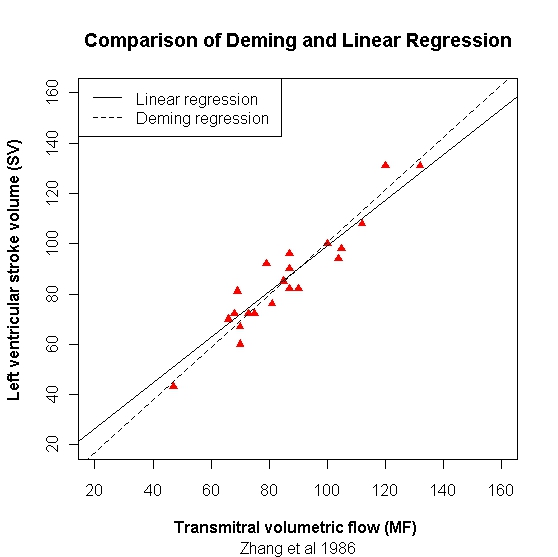
\includegraphics[width=130mm]{images/ZhangDeming.jpeg}
	\caption{Deming Regression For Zhang's Data}\label{ZhangDeming}
\end{figure}




% latex table generated in R 2.6.0 by xtable 1.5-5 package


%\begin{figure}[h!]
%	% Requires \usepackage{graphicx}
%	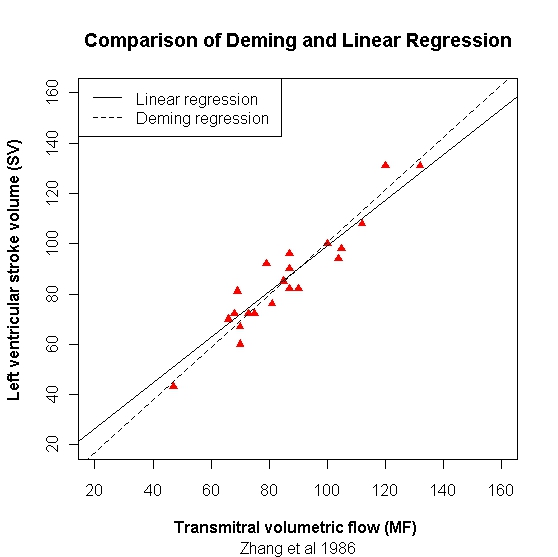
\includegraphics[width=130mm]{images/ZhangDeming.jpeg}
%	\caption{Deming Regression For Zhang's Data}\label{ZhangDeming}
%\end{figure}


This ratio can be estimated if multiple measurements were taken with each method, but if only one measurement was taken with each method, it can be assumed to be equal to one.


%\subsection{performance in the presence of oultiers}
%All least square estimation methods are sensitive to outliers.



Deming regression is undermined by several factors. Firstly it is computationally complex, and it requires specific software packages to perform calculations. Secondly, in common with all regression methods, Deming regression is vulnerable to outliers. Lastly, Deming regression is uninformative about the comparative precision of two methods of measurement. Most importantly \citet{CarollRupert} states that Deming's regression is acceptable only when the precision ratio ($\lambda$, in their paper as $\eta$) is correctly specified, but in practice this is often not the case, with the $\lambda$ being underestimated. This underestimation leads to an overcorrection for attenuation.

Several candidate models, with varying variance ratios may be fitted, and estimates of the slope and intercept are produced. However no model selection information is available to determine the best fitting model.

As noted before, Deming regression is an important and informative methodology in method comparison studies. For single measurement method comparisons, Deming regression offers a useful complement to LME models.

\section{Structural Equation Modelling}

Structural equation modelling is a statistical technique used for testing and estimating causal relationships using a combination of statistical data and qualitative causal assumptions. \citet{carrasco2004} describes the structural equation model is a regression approach that allows to estimate a linear 
regression when independent variables are measured with error.
The structural equations approach avoids the biased estimation of the slope and intercept that occurs in ordinary least square regression.

Several authors, such as \citet{lewis1991}, \citet{gkelly1985}, \citet{voelkel2005} and \citet{hopkins2004bias} advocate the use of SEM methods for method comparison. In \citet{hopkins2004bias}, a critique of the Bland-Altman plot he makes the following remark:

\begin{quote}
	\textit{What's needed for a comparison of two or more measures is a
		generic approach more powerful even than regression to model the
		relationship and error structure of each measure with a latent
		variable representing the true value.}
\end{quote}	

Hopkins also adds that he himself is collaborating in research utilising SEM and mixed effects modelling. \citet{gkelly1985} advised that \textit{the Structural equations model is used to estimate the linear relationship between new and standards method. The Delta method is used to find the variance of the estimated parameters} \citep{gkelly1985}.


Conversely \citet{BA99} also states that consider structural equation models to be inappropriate. However \citet{BA87} contends that it is unnecessary to perform elaborate statistical analysis, while also criticizing the SEM approach on the basis that it offers insights  on inter-method bias only, and not the variability about the line of equality. 
\begin{quote}
	\textit{However, it is quite wrong to argue solely from a lack of bias that two methods can be regarded as comparable...
		Knowing the data are consistent with a structural equation with a slope of 1 says something 
		about the absence of bias but nothing about the variability about Y = X (the difference between the measurements), which, as has already been stated, is all that really matters.}
\end{quote}

\citet{DunnSEME} highlights an important issue regarding using
models such as structural equatio modelling; the identifiability problem. This comes as a result of there being too many parameters to be estimated.
Therefore assumptions about some parameters, or estimators used,
must be made so that others can be estimated. For example, the ratio of the precision of both methods $\lambda=\frac{\sigma^{2}_{1}}{\sigma^{2}_{2}}$
must often be assumed to be equal to $1$ \citep{linnet98}. 

\citet{DunnSEME} considers techniques based on two methods with single measurements on each subject as inadequate for a serious study on the measurement characteristics of the methods, simply because there would not be enough data to allow for a meaningful analysis. There is, however, a contrary argument that in many practical settings it is very difficult to get replicate
observations when the measurement method requires an invasive medical
procedure.

%This application of the
%Grubbs method presumes the existence of this condition, and necessitates
%replication of observations by means external to and independent of the first
%means. The Grubbs estimators method is based on the laws of propagation of
%error. By making three independent simultaneous measurements on the same
%physical material, it is possible by appropriate mathematical manipulation of
%the sums and differences of the associated variances to obtain a valid
%estimate of the precision of the primary means. Application of the Grubbs
%estimators procedure to estimation of the precision of an apparatus uses
%the results of a physical test conducted in such a way as to obtain a series
%of sets of three independent observations.

\section{Model for Replicate Measurements}

The single measurement model can be generalized to the replicate measurement case, by additionally specifying replicate values. Let $y_{mir}$ be the $r-$th replicate measurement for item $i$ made by method $m$. Further to \citet{Barnhart} fixed effect can be expressed with a single term $\alpha_{mi}$, which incorporate the true value $\mu_i$.
\[ y_{mir} = \mu_{i} + \alpha_{m} + e_{mir}  \]
Combining fixed effects \citep{Barnhart}, we write,
\[ y_{mir} = \alpha_{mi} + e_{mir}.\]
The following assumptions are required
$e_{mir}$ is independent of the fixed effects with mean $\mbox{E}(e_{mir}) = 0$.
Further to \citet{Barnhart} between-item and within-item variances $\operatorname{Var}(\alpha_{mi}) = \sigma^2_{Bm}$ and $\operatorname{Var}(e_{mir}) = \sigma^2_{Wm}$		


\subsection{Carstensen's Model for Replicate Measurements}


%If the exact cause of disagreement between the two methods is not of interest, then the overall vaiability test $H_4$ %is an alternative to testing $H_2$ and $H_3$ separately.

\citet{BXC2008} develop their model from a standard two-way analysis of variance model, reformulated for the case of replicate measurements, with random effects terms specified as appropriate. 
For the replicate case, an interaction term $c$ is added to the model, with an associated variance component. Their model describing $y_{mir} $, again the $r$th replicate measurement on the $i$th item by the $m$th method ($m=1,2,$ $i=1,\ldots,N,$ and $r = 1,\ldots,n$), can be written as
\begin{equation}\label{BXC-model}
y_{mir}  = \alpha_{m} + \mu_{i} + a_{ir} + c_{mi} + \epsilon_{mir}.
\end{equation}

The fixed effects $\alpha_{m}$ and $\mu_{i}$ represent the intercept for method $m$ and the `true value' for item $i$ respectively. The random-effect terms comprise an item-by-replicate interaction term $a_{ir} \sim \mathcal{N}(0,\varsigma^{2})$, a method-by-item interaction term $c_{mi} \sim \mathcal{N}(0,\tau^{2}_{m}),$ and model error terms $\varepsilon_{mir} \sim \mathcal{N}(0,\varphi^{2}_{m}).$ All random-effect terms are assumed to be independent. For the case when replicate measurements are assumed to be exchangeable for item $i$, $a_{ir}$ can be removed. 



\citet{BXC2008} notes that, for $m=2$, separate estimates of $\tau^2_m$ can not be obtained. To overcome this, the assumption of equality, i.e. $\tau^2_1 = \tau^2_2$ is required.
\begin{equation}
y_{mir}  = \alpha_{m} + \mu_{i} + c_{mi} + e_{mir}, \qquad  e_{mi}
\sim \mathcal{N}(0,\sigma^{2}_{m}), \quad c_{mi} \sim \mathcal{N}(0,\tau^{2}_{m}).
\end{equation}
Based on this model, \citet{BXC2008} compute the limits of agreement as
\begin{equation}
\alpha_1 - \alpha_2 \pm 2 \sqrt{ \tau^2_1 +  \tau^2_2 +  \varphi^2_1 +  \varphi^2_2 }.
\end{equation}
This provides the basis of a modified approach to computing LOAs that will be reverted to later.
%Of particular importance is terms of the model, a true value for item $i$ ($\mu_{i}$). The fixed effect of Roy's model comprise of an intercept term and fixed effect terms for both methods, with no reference to the true value of any individual item. 
%A distinction can be made between the two models: Roy's model is a standard LME model, whereas Carstensen's model is a more complex additive model.



\bibliographystyle{chicago}
\bibliography{2017bib}
\end{document}

